\documentclass[../psets.tex]{subfiles}

\pagestyle{main}
\renewcommand{\leftmark}{Problem Set \thesection}

\begin{document}




\section{Applications of Molecular Orbitals}
\marginnote{9/25:}The questions pertain to the material we have covered from Introduction (Sep 5) to Pericyclic Reactions (Sep 19). For the molecular orbital (MO) diagrams, please draw the MOs with appropriate energy levels, fill in the electrons, and draw cartoons that illustrate the orbital
interactions.
\begin{enumerate}
    \item The geometry of \ce{PMe3} (\textbf{1}) is known to be pyramidal.
    \begin{center}
        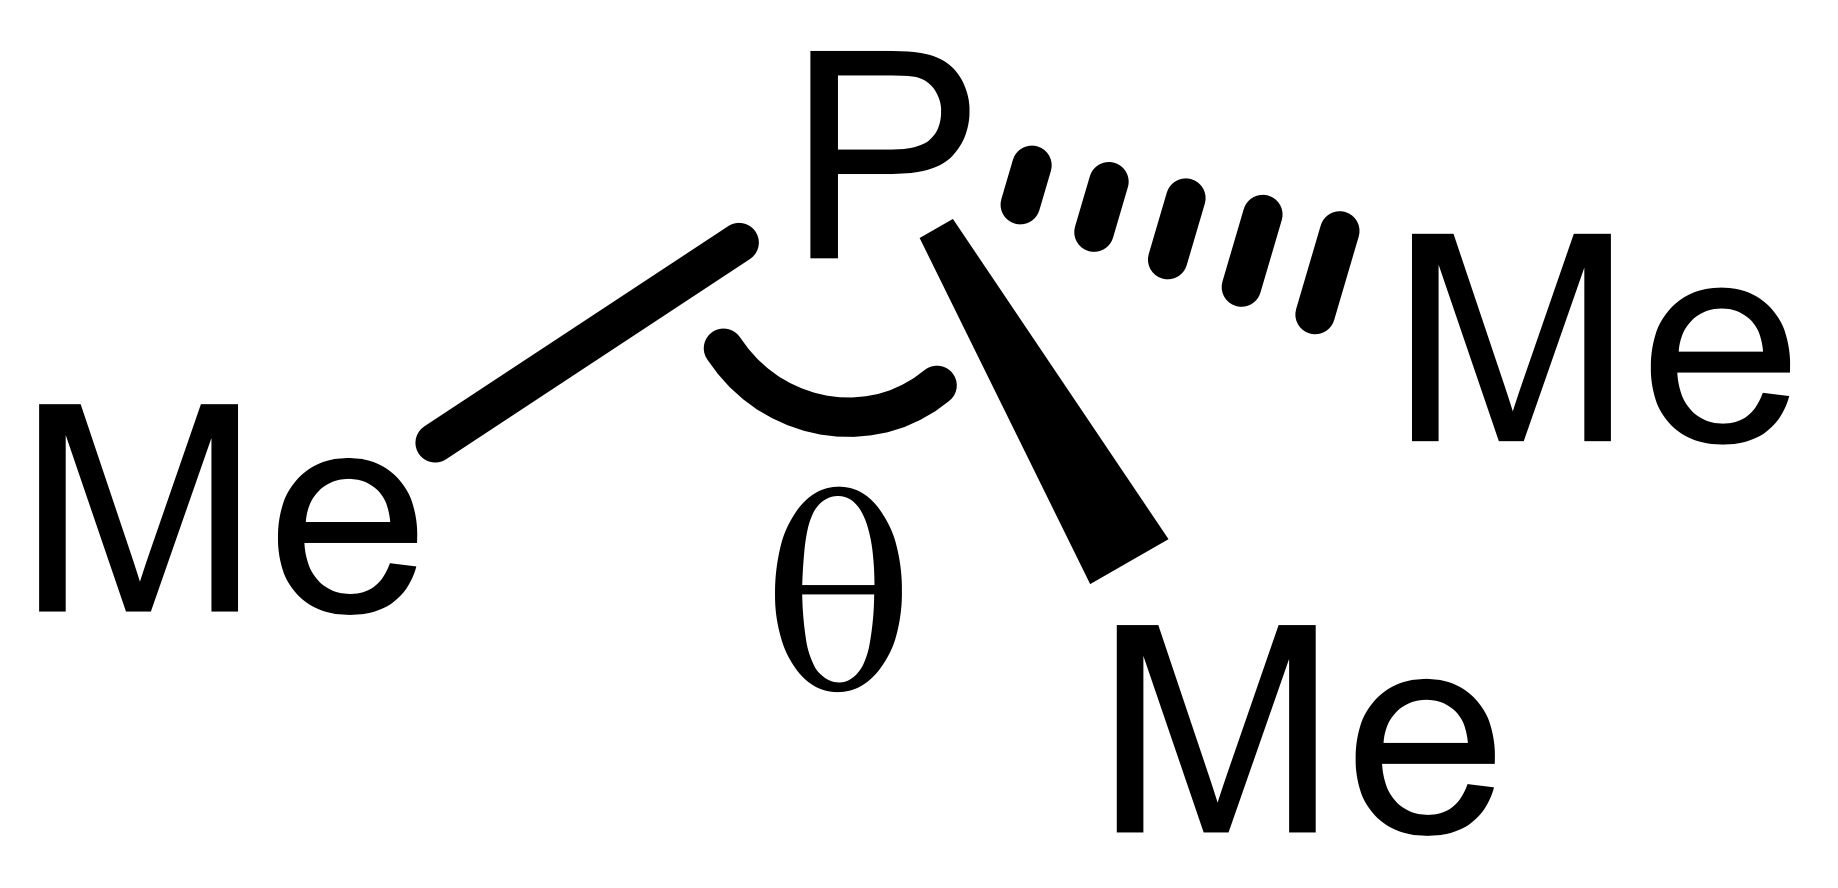
\includegraphics[width=0.12\linewidth]{PSet1F1.png}\\
        \textbf{1}
    \end{center}
    A qualitative MO diagram for the frontier orbitals of \ce{PMe3} can be drawn as follows.
    \begin{center}
        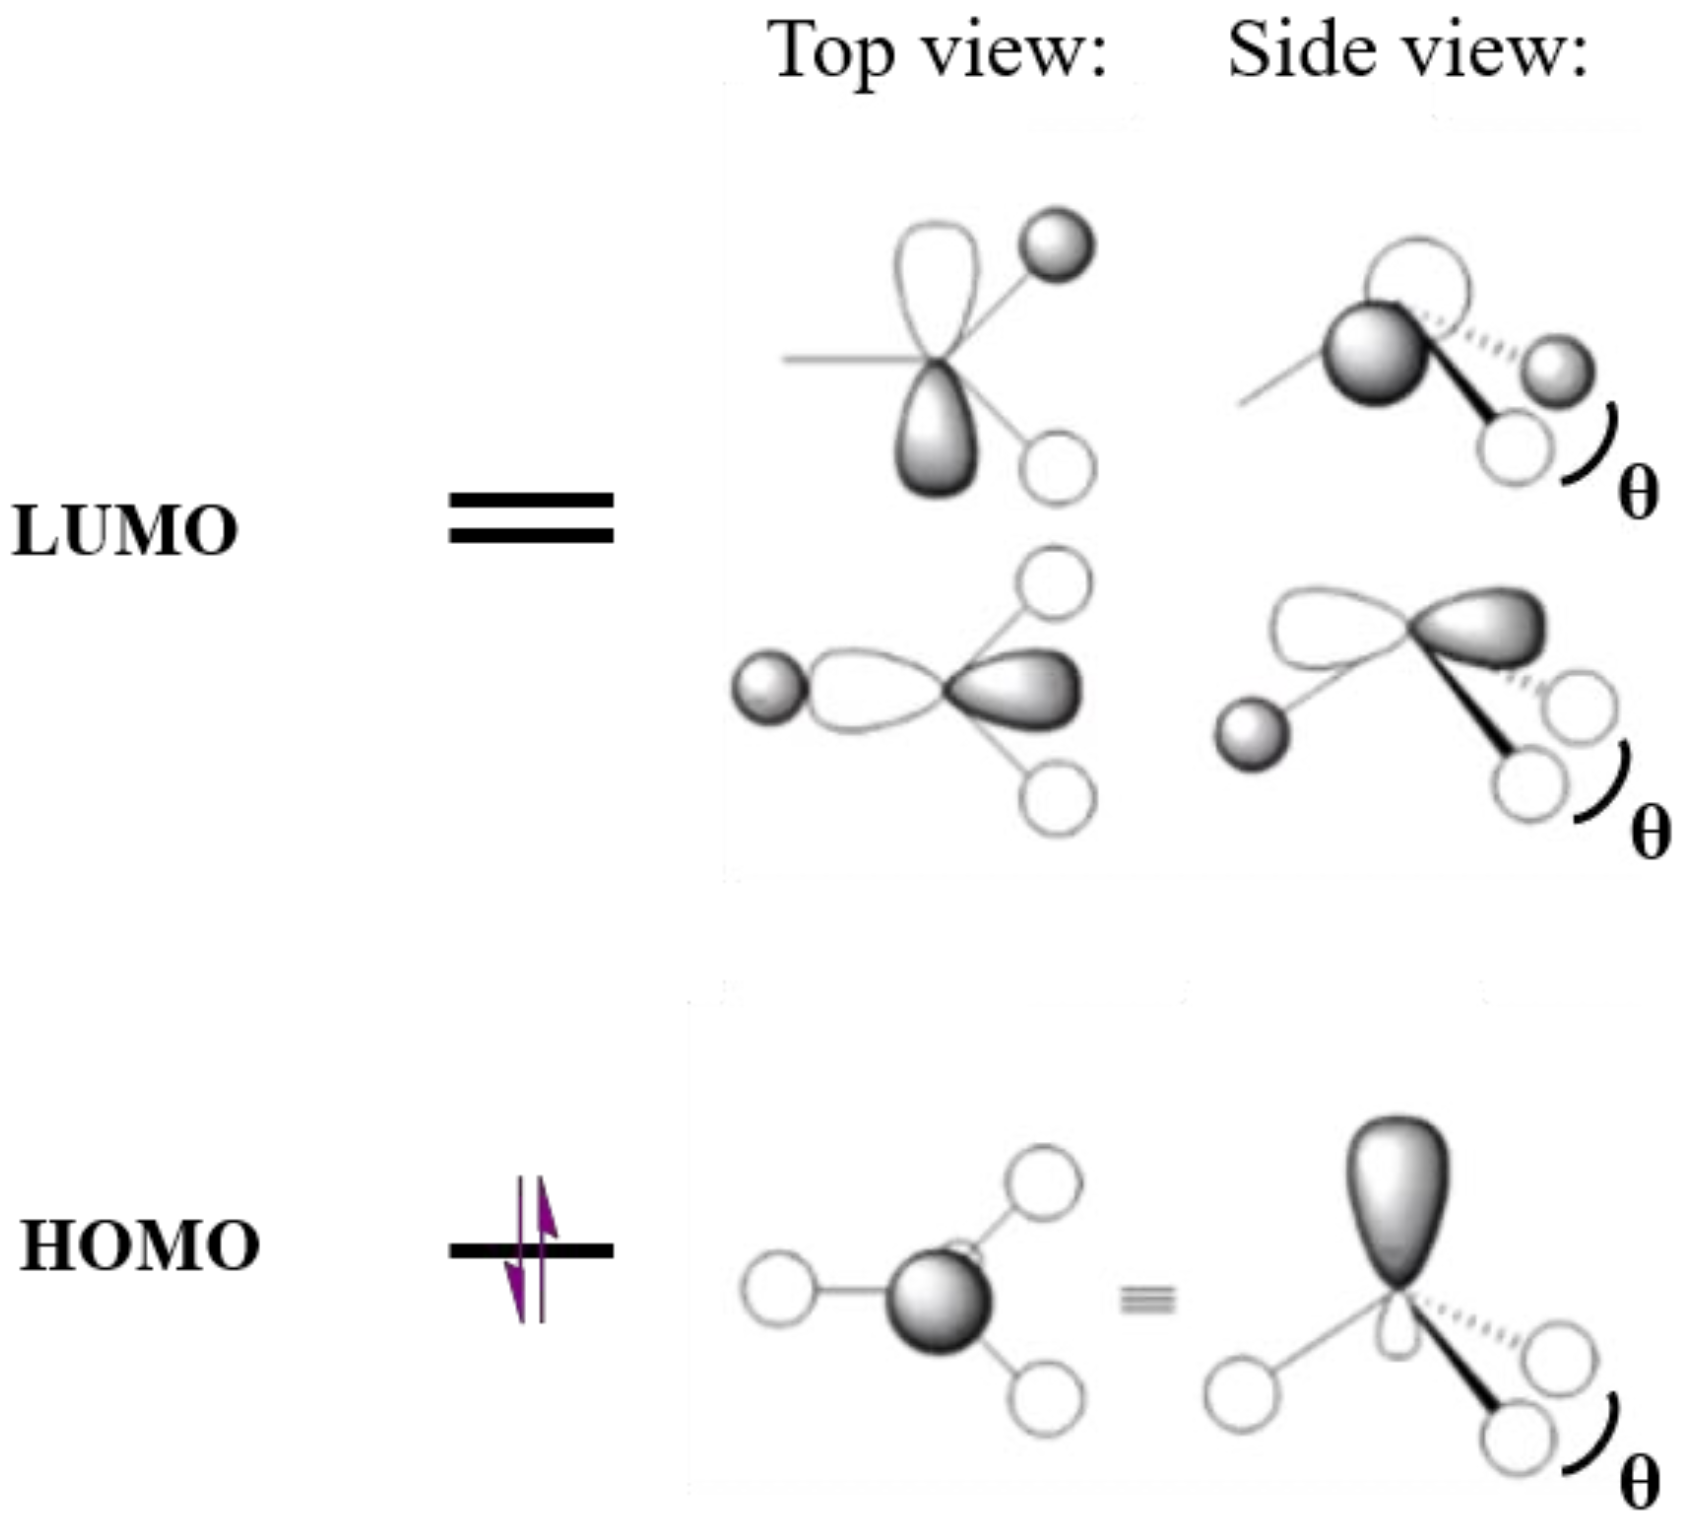
\includegraphics[width=0.4\linewidth]{PSet1F2.png}
    \end{center}
    \begin{enumerate}
        \item How will the energies of the frontier orbitals change if we decrease one \ce{C-P-C} angle, denoted as $\theta$, by symmetrically moving the two methyl groups closer to each other? Draw a Walsh diagram for the frontier orbitals to explain. Assume that the bond lengths are unchanged.
        \item How will the energies of the frontier orbitals change if we instead increase $\theta$ while maintaining the bond lengths? Draw a Walsh diagram for the frontier orbitals to explain.
        \item Rank the relative nucleophilicity and electrophilicity of the following molecules, and rationalize your hypotheses.
        \begin{center}
            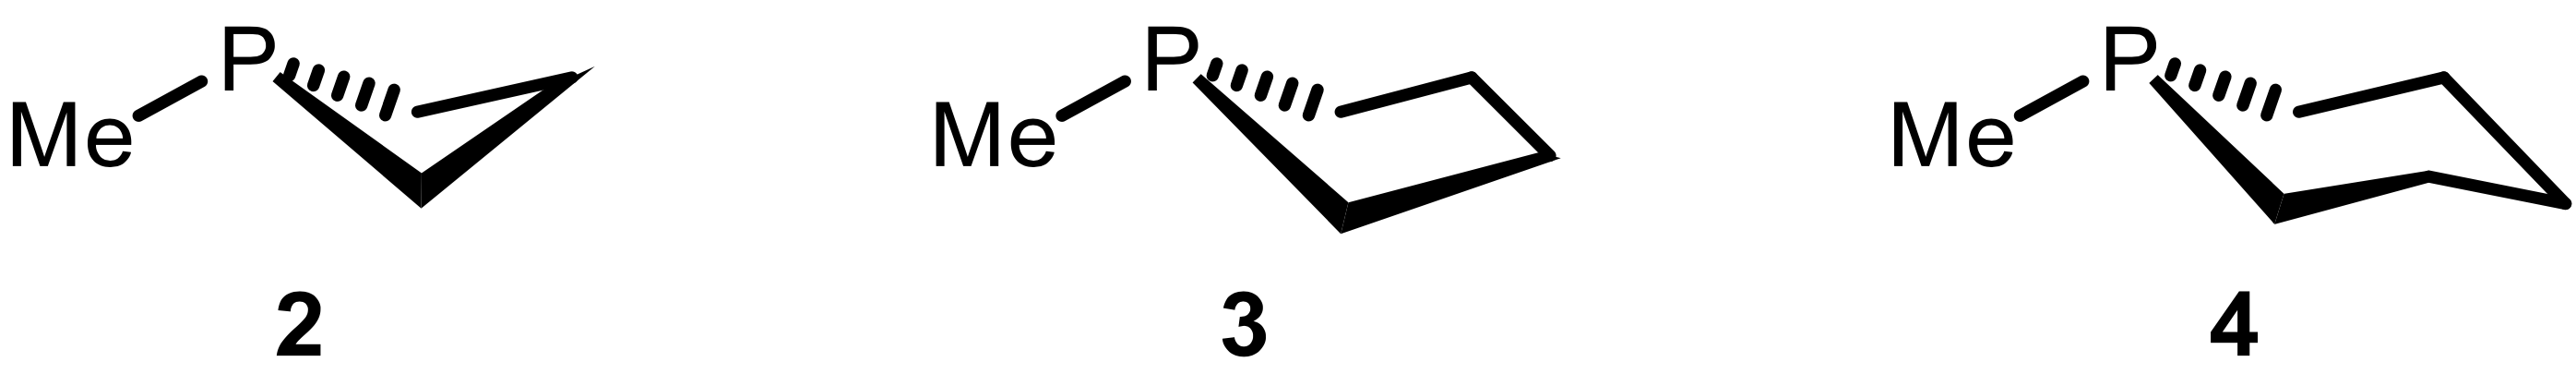
\includegraphics[width=0.5\linewidth]{PSet1F3.png}
        \end{center}
    \end{enumerate}
    \item Consider the combination of two allyl fragments (\textbf{1}) joined at the center carbons, leading to diradical (\textbf{2}).
    \begin{center}
        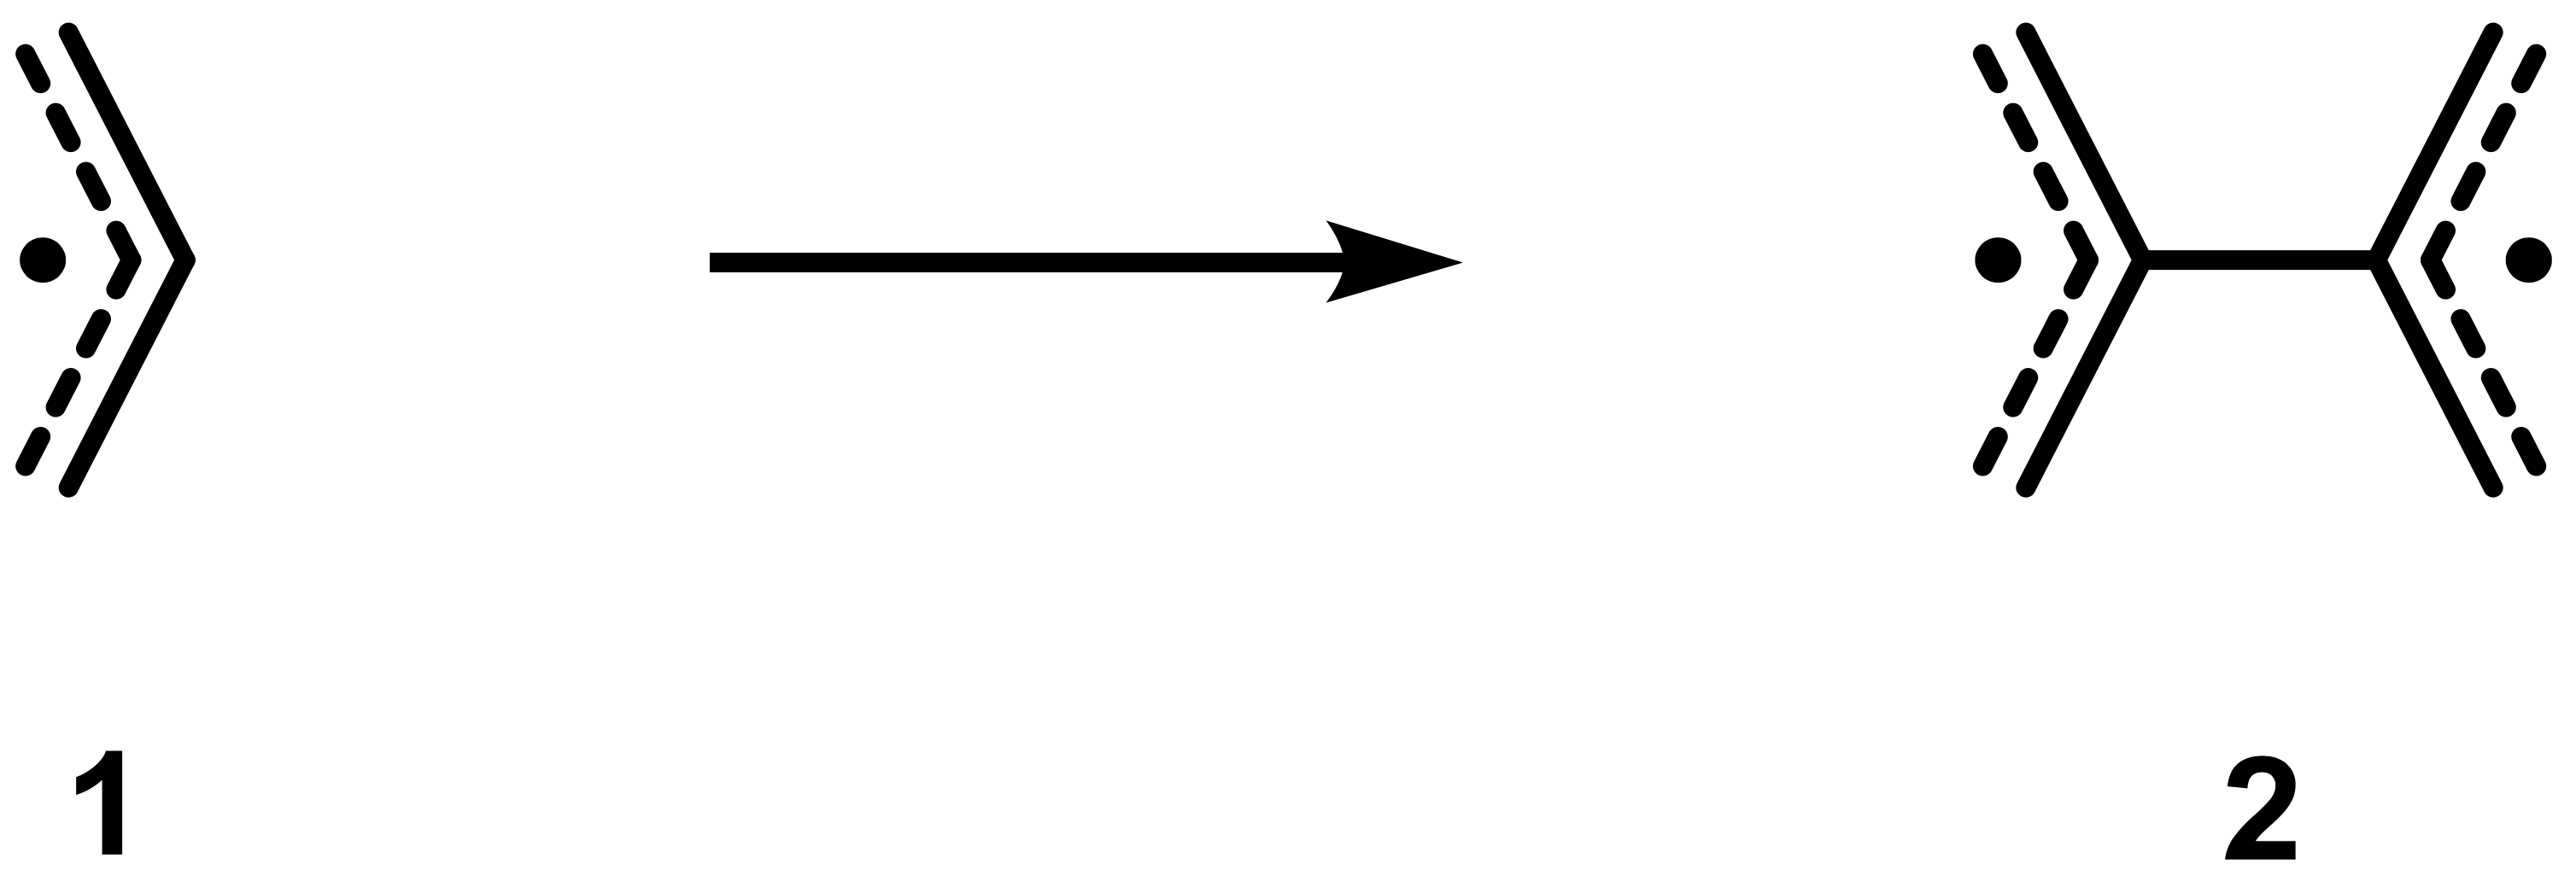
\includegraphics[width=0.35\linewidth]{PSet1F4.png}
    \end{center}
    \begin{enumerate}
        \item Construct a $\pi$ MO interaction diagram for \textbf{2} that predicts the symmetries of the combined MOs and their energies relative to carbon $p$-orbitals. Please assume that only interactions between AOs on \underline{adjacent atoms} are significant.
        \item Can the two radical centers delocalize via resonance? Explain using the MO diagram from part (a).
    \end{enumerate}
    \item Predict the stereochemistry of the product and rationalize your answer based upon MO theory.
    \begin{center}
        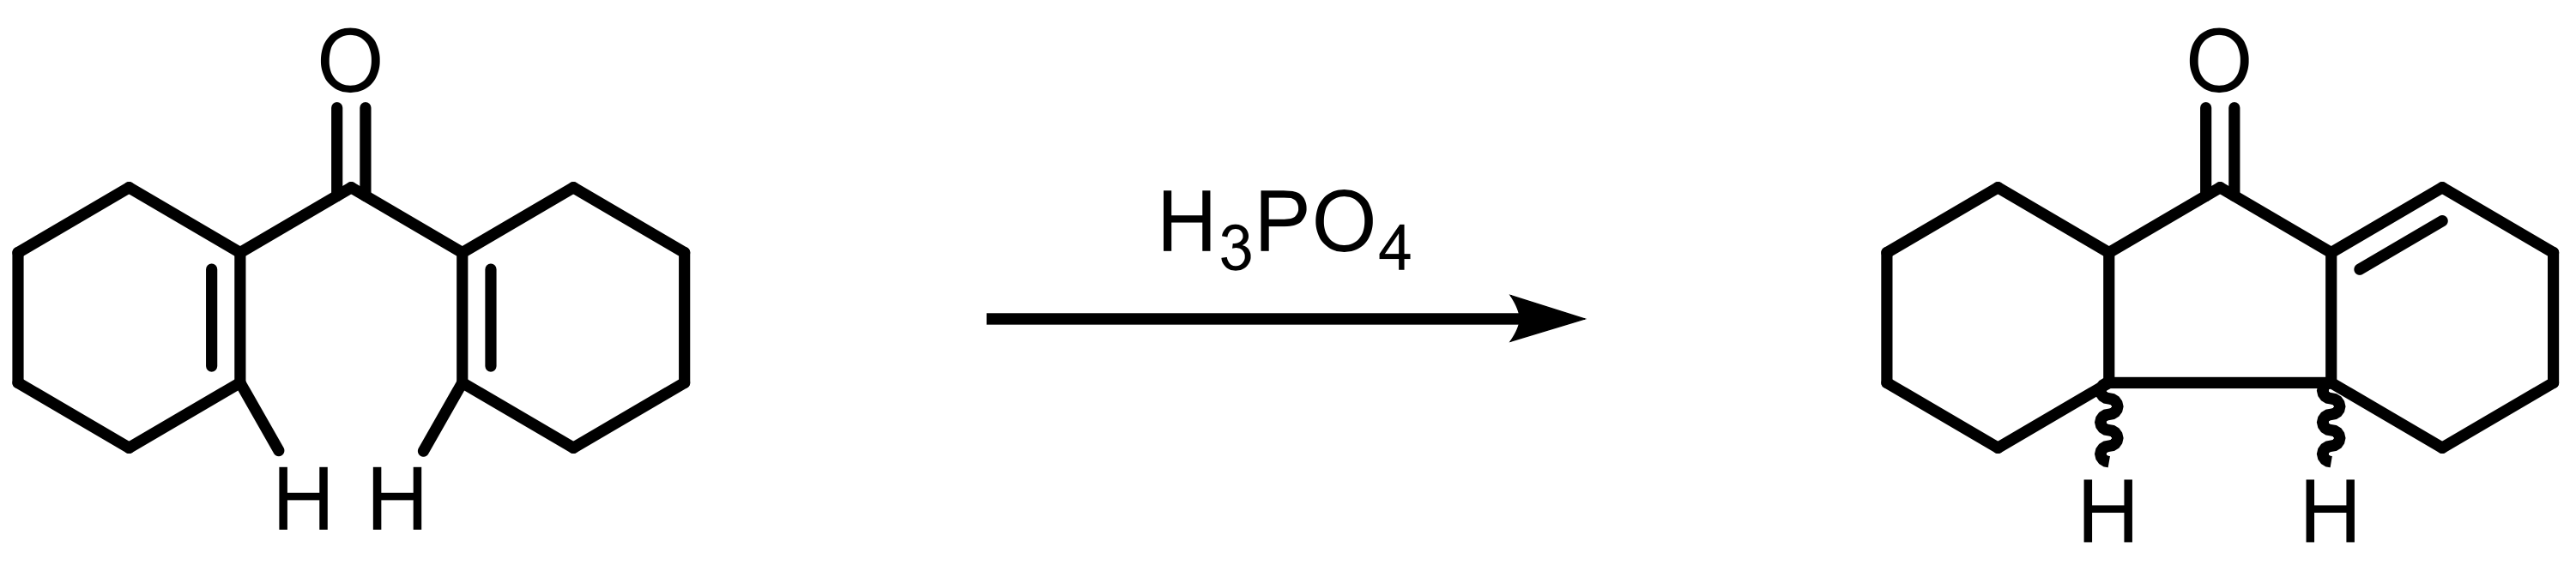
\includegraphics[width=0.5\linewidth]{PSet1F5.png}
    \end{center}
    \item Norbornadiene is known to be more reactive towards electrophiles than norbornene.
    \begin{center}
        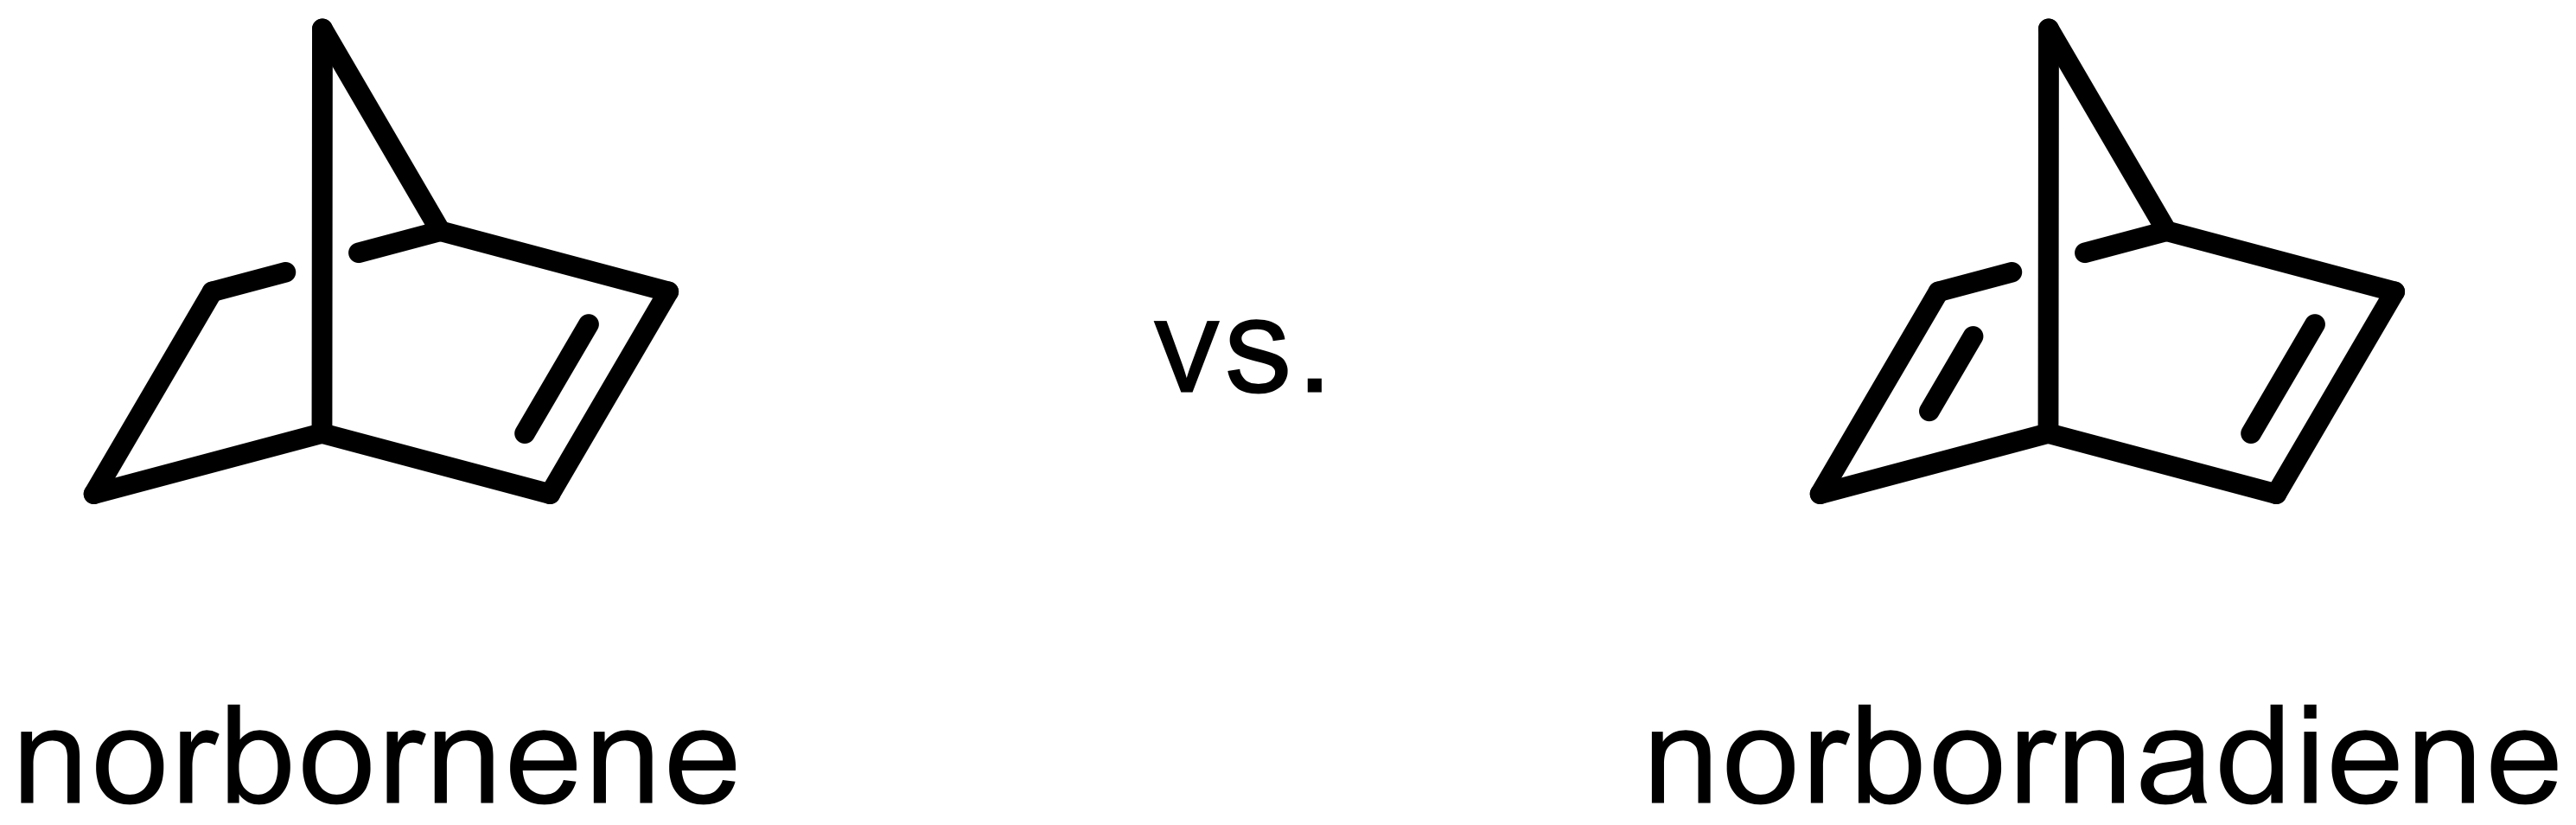
\includegraphics[width=0.37\linewidth]{PSet1F6.png}
    \end{center}
    \begin{enumerate}
        \item Rationalize this difference using an MO diagram.
        \item Norbornadiene derivatives can be converted to quadricyclane derivatives under UV irradiation. Quadricyclanes are highly strained molecules, yet they are thermally stable.
        \begin{center}
            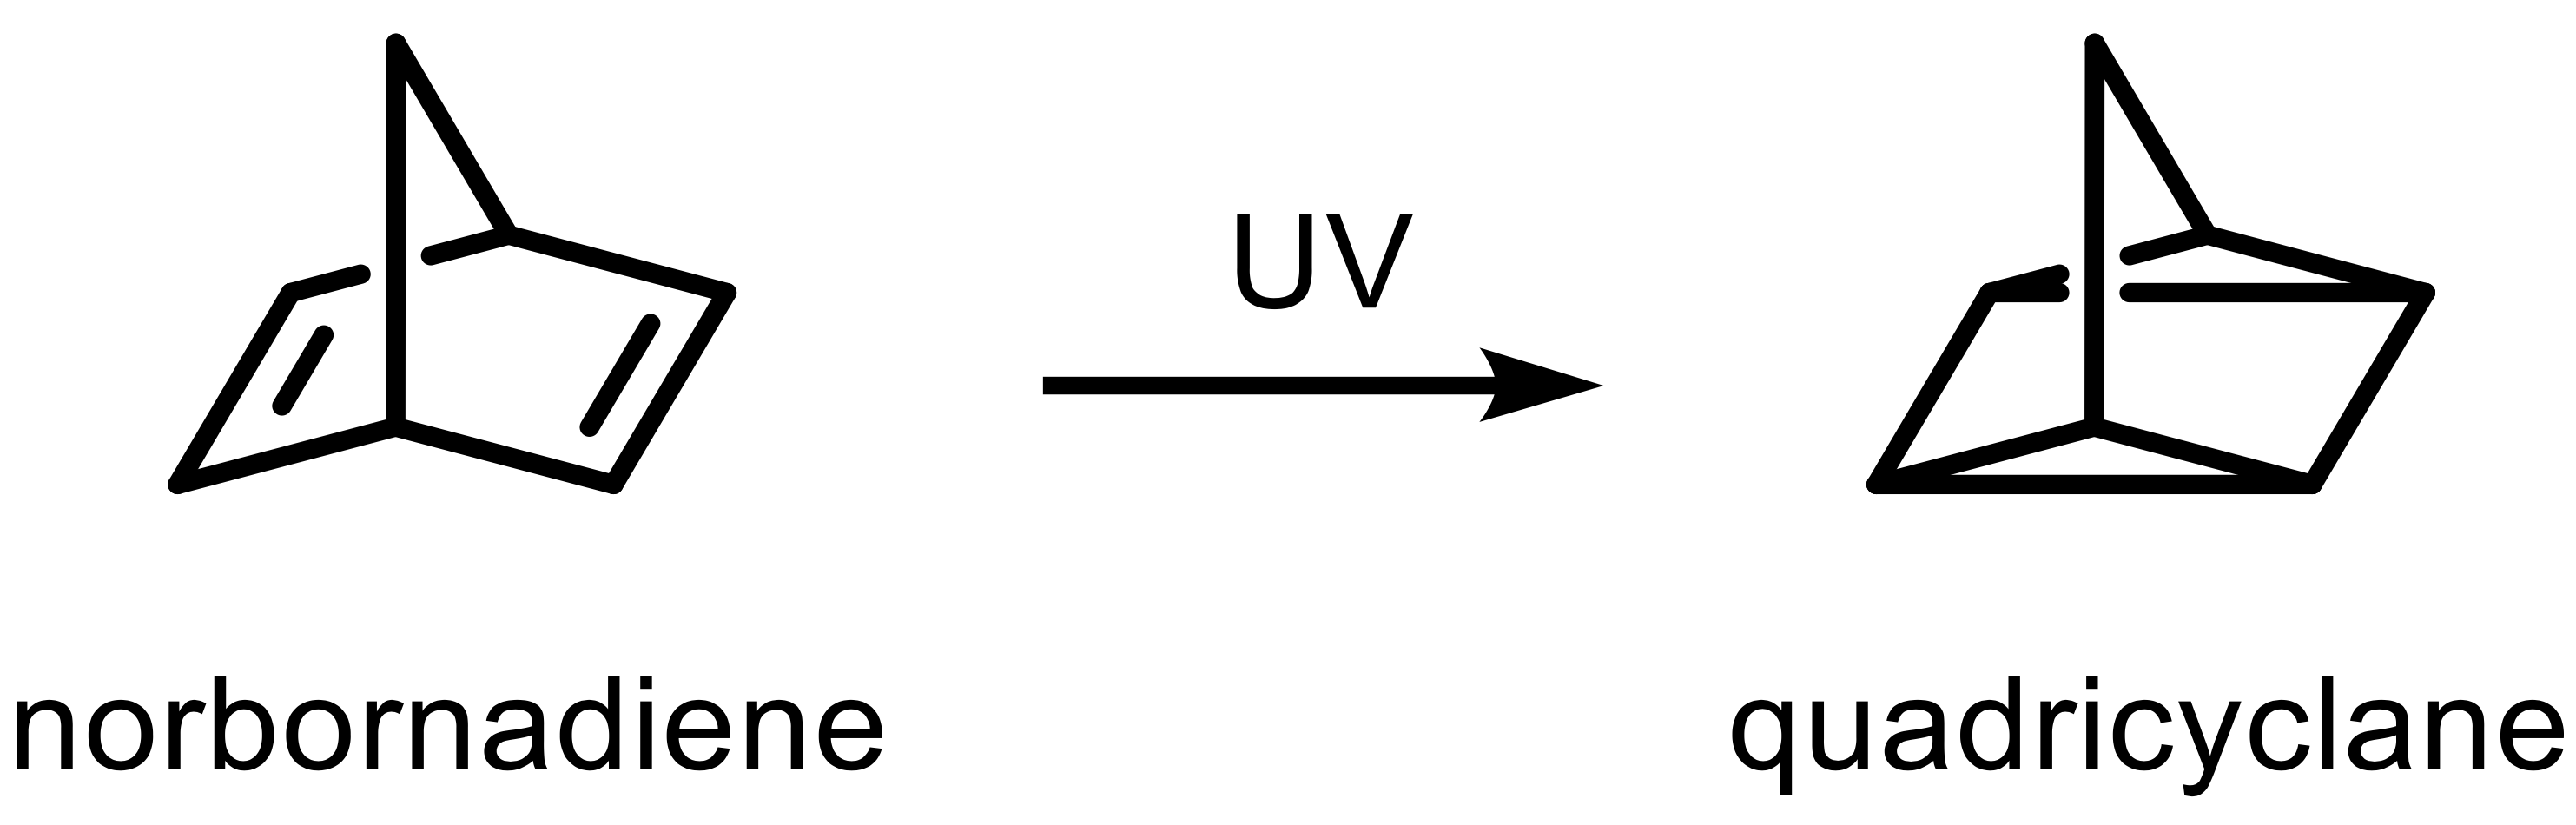
\includegraphics[width=0.4\linewidth]{PSet1F7.png}
        \end{center}
        Provide a frontier MO analysis to explain why quadricyclane is thermally stable.
    \end{enumerate}
    \item Please use computational tools to complete this question. We will be using a browser-based quantum chemistry platform (\href{https://rowansci.com/}{Rowan}) for this course.
    \begin{enumerate}
        \item Create an account on Rowan (\url{https://rowansci.com/}) using your MIT email.
        \begin{itemize}
            \item To learn how to submit a job on Rowan, please watch this video tutorial: \url{https://docs.rowansci.com/web-interface/run-a-simple-job} and/or read this overview: \url{https://docs.rowansci.com/web-interface/submit/geometry-optimization}.
            \item More information on how to use Rowan (as well as additional tools) can be found here: \url{https://docs.rowansci.com/web-interface}.
        \end{itemize}
        \item Ethane (\ce{H3CCH3}).
        \begin{enumerate}
            \item Using any means, build a molecular model for ethane in Rowan. Then, perform a geometry optimization using the PBE0 functional and the def2-SVP basis set. Take a screenshot of the webpage before submitting the job and paste it here.
            \begin{itemize}
                \item Note: this job should not take more than 1 minute to run (not including queue time). If it takes significantly longer, consider adjusting your initial bond lengths/angles.
            \end{itemize}
            \item Convert the optimized structure into Cartesian (XYZ) coordinates and paste them here.
            \item What is the calculated optimized \ce{C-C} bond distance? What is the \ce{H-C-H} bond angle(s)?
        \end{enumerate}
        \item Ethyl cation (\ce{H3CCH2+}).
        \begin{enumerate}
            \item Using any means, build a molecular model for the ethyl cation in Rowan. Then, perform a geometry optimization using the PBE0 functional and the def2-SVP basis set. Take a screenshot of the webpage before submitting the job and paste it here.
            \begin{itemize}
                \item Note: this job should not take more than 1 minute to run (not including queue time). If it takes significantly longer, consider adjusting your initial bond lengths/angles.
            \end{itemize}
            \item Convert the optimized structure into Cartesian (XYZ) coordinates and paste them here.
            \item What is the calculated optimized \ce{C-C} bond distance? What is the \ce{H-C-H} bond angle(s)?
        \end{enumerate}
        \item Now, using qualitative MO arguments based on your calculations, discuss at least two factors contributing to the differing \ce{C-C} bond lengths in ethane vs ethyl cation.
    \end{enumerate}
\end{enumerate}




\end{document}